\section{Background}
\subsection{SIMD}
\subsection{Leros}
In order to avoid carrying out redundant work, a decision was made to utilise an
existing solution as a base development. The advantages were twofold; not only
did it allowed for much faster development, but had already been tested by many
people. Opencores\footnote{
http://www.opencores.com
}
is a large open-source hardware community, well-known for its collection of hardware solutions for
FPGAs and ASICs, in both VHDL and Verilog. Our requirements called for a VHDL
microcontroller, of which there were many to choose from. Other critera included
simplicity of code, small code size, and a RISC architecture. One project stood out
after applying these critera, named the \emph{Leros} microcontroller after the
Greek Island Leros \cite{cite:TODO}.  The Leros MCU is a 16-bit
processor optimized for FPGAs \cite{cite:TODO}, and was selected for use in this
project.

 It is a stable
project and can even be programmed in a restricted subset of Java. It is licenced
under the permissive BSD licence and has been tested under the Xilinx toolchain.
Leros' architecture is a pipelined 16-bit accumulator processor\ref{cite:TODOpdf},
with instructions exectuted in a single cycle.

The accumulator architeuectur made Leros an attractive option for this project.

\begin{figure*}[h]
\center
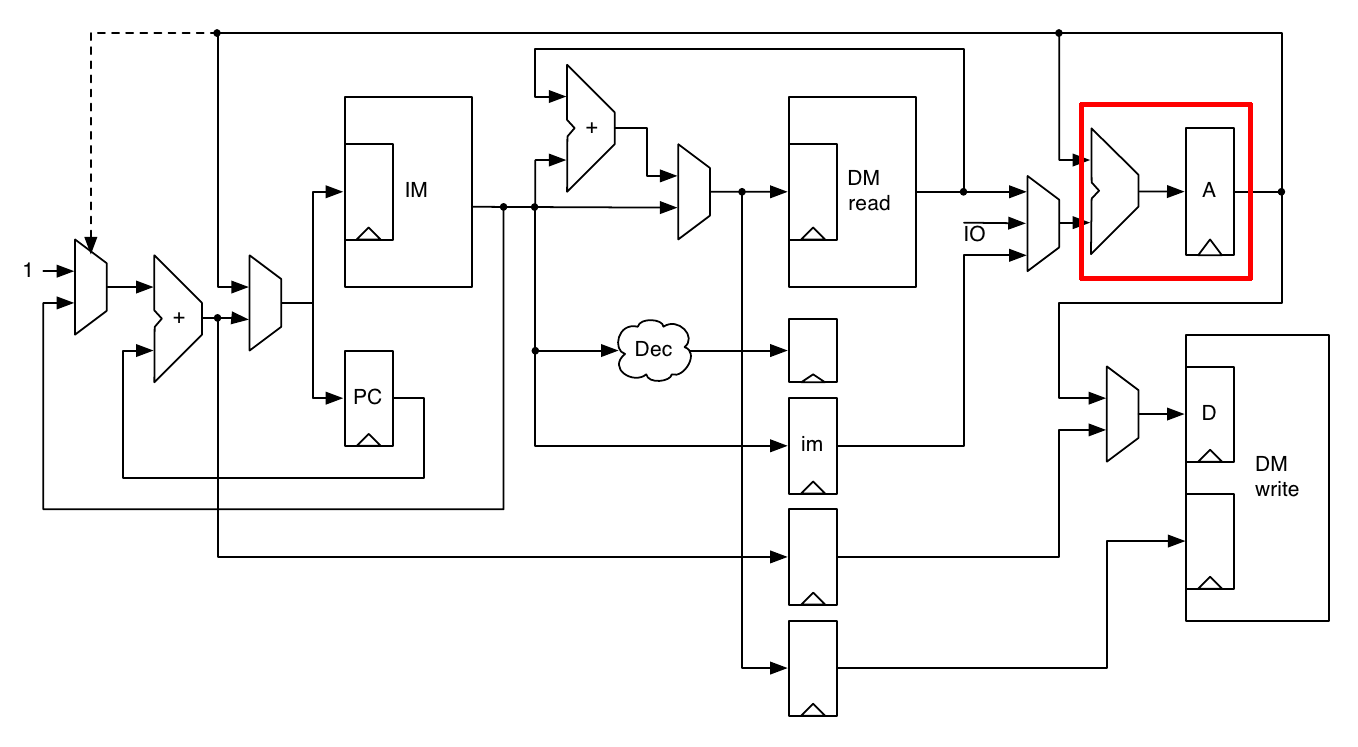
\includegraphics[width=0.9\textwidth]{images/leros-system}
\caption{Leros pipeline. The section of the design to be multiplied has been
highlighted in red. Original image from \cite{cite:TODO-pdf}.
}
\label{fig:leros-system}
\end{figure*}
